\subsection{概要}

訓練データセットを $\mathcal{D} = \{(\mathbf{X}_n, \mathbf{Y}_n)\}_{n=1}^{N}$ とする.
ここで,$N$ は訓練画像の総数,$\mathbf{X}_n \in \mathbb{R}^{H \times W \times C}$ は $n$ 番目の入力画像($C$はチャンネル数),
$\mathbf{Y}_n = \{y_{n,i,j}\}_{i,j} \in \mathbb{R}^{H \times W}$ は対応する正解マスクである.
MC Dropout による不確実性推定では,各画像に対して $T$ 回の確率的推論を行う.
$t$ 回目の推論($t \in \{1, \ldots, T\}$)における予測確率マップを $\hat{\mathbf{Y}}_n^{(t)} = \{\hat{y}_{n,i,j}^{(t)}\}_{i,j}$ と表記する.

図\ref{method} に提案手法の概要を示す.
本手法の設計は,主に以下の2つの観点に基づいている.
第一に,学習サンプルに対する難易度評価を,学習プロセスの中で動的に更新する点である.
画像の難易度は絶対的なものではなく,モデルの学習進捗によって変化する相対的なものであるため,
現在のモデルの状態に基づいて難易度を逐次再評価することで,
その時点でのモデルにとって確信を持てない画像に学習を集中できる.
第二に,難易度の定量化指標として,認識的不確実性が適している点である.
認識的不確実性は「モデルの知識不足」に起因するため,モデルが未学習のパターンや判断に迷っている領域を直接的に反映するため,
ノイズに影響されることなく,学習によって改善可能な「モデルにとってどれくらい確信を持てないか」を適切に定量化することが可能となる.

提案法では,学習中各画像に対して $\tau$ エポックごとに MC Dropout を用いて画像毎に複数枚推論を行い,予測のばらつきから不確実性を定量化する.
この不確実性情報は,モデルがその画像のセグメンテーションにおいてどの程度の確信を持てないかを反映する.
その後,この不確実性情報を画像単位に集約し,PolyDice Loss の形状を動的に制御することで,難しい画像には急峻な勾配を,簡単な画像には緩やかな勾配を与える.
更新された $\epsilon$ を次の $\tau$ エポック間の学習に適用することで,学習の進行度に応じて最適化の重み付けを動的に変化させる適応的学習を実現する.

\clearpage

\begin{figure}
    \includegraphics[width=\columnwidth]{figure/method.pdf}
    \caption{Overview of the proposed adaptive learning framework.
The process consists of two phases: uncertainty estimation and adaptive training. Every $\tau$ epochs, the model evaluates image difficulty using MC Dropout and updates the loss shape parameter $\epsilon$. This dynamic control assigns steeper gradients to harder samples, enabling difficulty-aware optimization.}
    \label{method}
\end{figure}

\clearpage

\subsection{不確実性に基づく画像難易度の定量化}

\subsubsection{学習中のMC Dropout推論}

提案法では,学習プロセスを初期学習期間と適応的学習期間の2段階に分割する.
エポック $1$ から $E_0 - 1$ までの期間は初期学習期間とし,損失形状パラメータ $\epsilon$ を$0$に固定して学習を行う.
この期間を設ける理由は,学習初期のモデルは特徴表現が未成熟であり,この段階での不確実性は画像の本質的な難易度よりもモデルの初期化に依存するためである.
$E_0$はモデルが基礎的なセグメンテーション能力を獲得するのに十分なエポック数として設定する.

適応的学習期間($e \geq E_0$)においては,周期 $\tau$ ごとに不確実性の再評価と $\epsilon$ の更新を行う.
すなわち,更新は $e \in \{E_0, E_0+\tau, E_0+2\tau, \ldots\}$ を満たすエポックの学習開始前に実行される.
更新の際は,その時点のモデルパラメータ $\mathbf{W}$ を固定し,訓練データの各画像 $\mathbf{X}_n$ に対して Dropout 率 $p \in (0,1)$ で $T$ 回の確率的推論を行う.
得られる予測集合を $\{\hat{\mathbf{Y}}_n ^ {(t)}\}_{t=1}^{T}$ とする:
%
\begin{equation}
    \hat{\mathbf{Y}}_n ^ {(t)} = f_{\mathbf{W}}(\mathbf{X}_n; \mathbf{z}^{(t)}), \quad \mathbf{z}^{(t)} \sim \text{Bernoulli}(1-p)
\end{equation}
%
ここで,$\mathbf{z}^{(t)}$ は $t$ 回目の推論における Dropout マスクであり,$\hat{\mathbf{Y}}_n ^ {(t)}$ はその予測確率マップである.
この確率的推論により得られる予測のばらつきから,モデルの認識的不確実性を定量化する.

\subsubsection{ピクセル単位の不確実性指標の計算}
MC Dropoutによって得られた $T$ 枚の予測画像に対し,ピクセル単位の不確実性指標として
認識的不確実性を直接捉えることができる相互情報量 $I_{n, i, j}$ を計算する.

\begin{equation}
    I_{n, i, j} = \underbrace{H\left( \frac{1}{T} \sum_{t=1}^{T} \hat{y}_{n, i,j}^{(t)} \right)}_{\text{Entropy of Mean}} - \underbrace{\frac{1}{T} \sum_{t=1}^{T} H\left( \hat{y}_{n, i,j}^{(t)} \right)}_{\text{Mean of Entropy}}
\end{equation}

ここで,$H(p)$ は2値分類におけるバイナリ・エントロピー関数であり,次式で定義される.

\begin{equation}
    H(p) = -p \log p - (1-p) \log (1-p)
\end{equation}

相互情報量はモデルの予測に付随する不確実性を評価し,その依拠する要因を分離する指標として広く用いられている.
$T$ 回の推論結果を平均化した後の予測分布に対する不確実性であり,データとモデルの両方に由来する不確実性を示す予測エントロピーから,
個々の推論における不確実性の平均であり,
データ固有のノイズや曖昧さに由来する偶然的不確実性を示す期待エントロピーを減ずることで,認識的不確実性を定量化できる.
値が高い領域はモデルが十分に学習できていないことを示唆する.

\subsubsection{画像単位への集約}
ピクセル単位の相互情報量から外れ値を除去した後の平均値を,画像全体の難易度指標として定量化する.
医用画像セグメンテーションでは,背景領域が画像の大部分を占める一方で,関心領域である病変部は極めて小さいクラス不均衡が存在する.
背景領域は一般に推論が容易であり,その不確実性は極めて低い値をとる傾向がある. そのため,画像全体で不確実性の平均を算出すると,
大量の背景画素による低い値が難易度指標全体を支配してしまい,本来捉えるべき病変部の局所的な難易度を適切に定量化できない可能性がある.\\
したがって,病変検出の難易度を鋭敏に反映させるため,本手法では正解画像における病変領域に限定して相互情報量の平均を算出する.
画像領域全体を $\Omega_n$,正解マスクにおける陽性領域の画素集合を $\mathcal{P}_n = \{(i,j) \in \Omega \mid y_{i,j} = 1\}$ とする.
ここで,算出される相互情報量には突発的なノイズや極端な外れ値が含まれる可能性があり,これらが難易度指標の定量化を不安定にさせる要因となる.
そのため,スコアの算出に先立ち,統計的な外れ値除去を行う.
具体的には,領域 $\mathcal{P}_n$ 内の相互情報量の平均を $\mu_{\mathcal{P}_n}$,標準偏差を $\sigma_{\mathcal{P}_n}$ とし,有効な画素集合 $\mathcal{P}_n'$ を以下のように定義する.
\begin{equation}
    \mathcal{P}_n' = (i,j) \in \left\{\mathcal{P}_n \mid \mu_{\mathcal{P}_n} - 2\sigma_{\mathcal{P}_n} \leq I_{n, i, j} \leq \mu_{\mathcal{P}_n} + 2\sigma_{\mathcal{P}_n} \right\}
\end{equation}
ここで,閾値として $2\sigma_{\mathcal{P}_n}$ を採用した根拠は,統計的な信頼区間の考え方に基づく.
相互情報量の分布が正規分布に近似できると仮定した場合,平均値を中心とした $\pm 2\sigma$ の範囲内には全データの約 $95\%$ が含まれる.
したがって,この範囲外のデータを棄却することで,統計的に特異な極端値(外れ値)を効果的に除去しつつ,病変部の主要な特徴を反映したロバストな難易度推定が可能となる.
この有効集合 $\mathcal{P}_n'$ を用いて,画像全体の難易度スコア $D_n$ は次式で算出される.
\begin{equation}
    D_n = \frac{1}{|\mathcal{P}_n'|} \sum_{(i,j) \in \mathcal{P}_n'} I_{n, i,j}
\end{equation}
ここで,$|\mathcal{P}_n'|$ は外れ値除去後の陽性領域の画素数を表す.
なお,陽性領域が存在しない画像については,$D_n = 0$ とする.

次に,各サンプルの相対的な難易度を決定するため,データセット全体の難易度スコア分布に基づいて正規化を行う.
ここでの目的は,画像毎の数値的なスケールの差異を吸収し,各画像が分布全体の中で相対的にどの程度難しいかを評価することである.
データセット全体のスコア集合$\{D_n\}_{n = 1} ^ N$に対し, $q$ パーセンタイル値を $D_q$,標準偏差を $\sigma_D$ とすると,正規化されたスコアは次のように計算される.

\begin{equation}
    D_{n} ^ {\text{norm}} = \frac{D_n - D_{q}}{\sigma_D + \delta}
\end{equation}
ここで,$\delta > 0$ は数値的安定性のための微小定数である.
$D_q$ による減算は,後述する制御関数への入力を合わせるための中心化をする役割を持つ.
分布の平均値ではなく$q$パーセンタイル値を用いることで,容易なサンプルが多数を占める分布においても,
外れ値の影響を受けずに難易度の基準点を柔軟に設定できる.
$\sigma_D$ による除算は尺度の統一であり,
制御関数の感度がデータセットごとの不確実性のスケールに依存しないように調整する役割を持つ.

\subsection{適応的損失形状制御}

\subsubsection{制御関数の設計}
得られた難易度指標 $D_{n} ^ {\text{norm}}$ に基づき,PolyDice-1 Loss の形状パラメータ $\epsilon$ を動的に更新する.
更新式には以下のシグモイドベースの制御関数を用いる.

\begin{equation}
    \epsilon = \epsilon_{\text{min}} + (\epsilon_{\text{max}} - \epsilon_{\text{min}}) \sigma(k \cdot D_{n} ^ {\text{norm}})
\end{equation}
ここで,$\sigma(x) = (1 + e^{-x})^{-1}$標準シグモイド関数,$k > 0$ はパラメータであり,$\epsilon_{\text{min}}, \epsilon_{\text{max}}$ は $\epsilon$ の変動範囲である.

本手法でシグモイド関数を採用する理由は,有界性と滑らかさにある.
ステップ関数のような急激な切り替えは学習の安定性を損なう恐れがあり,
線形関数ではパラメータ$\epsilon$が適切な範囲$[\epsilon_{\text{min}}, \epsilon_{\text{max}}]$ を逸脱する可能性がある.
シグモイド関数を用いることで,難易度が低い領域から高い領域への遷移を滑らかに行いつつ,出力値を常に所定の範囲内に厳密に制約することが可能となる.
パラメータ $k$ は関数の応答感度を制御し,図\ref{sigmoid} に示すようにその値が大きいほど難易度判定の境界が急峻になり,小さいほど滑らかな遷移となる.

この制御により,難しい画像($D_{n} ^ {\text{norm}}$が大きい)に対しては,大きな$\epsilon$を割り当て,
損失関数の勾配を急峻にする.これは,同じ予測誤差に対して
より大きな損失値と勾配を与えることを意味し,結果として難しい画像からの学習信号が相対的に強化される.
一方,すでに十分に学習できている簡単な画像には小さな$\epsilon$を割り当て,過学習を防ぎつつ学習リソースを難しい画像に集中させる.
更新された $\epsilon$ は学習に適用され,これによりモデルは困難な画像の学習を重点的に行うことが可能となる.

\clearpage

\begin{figure}
    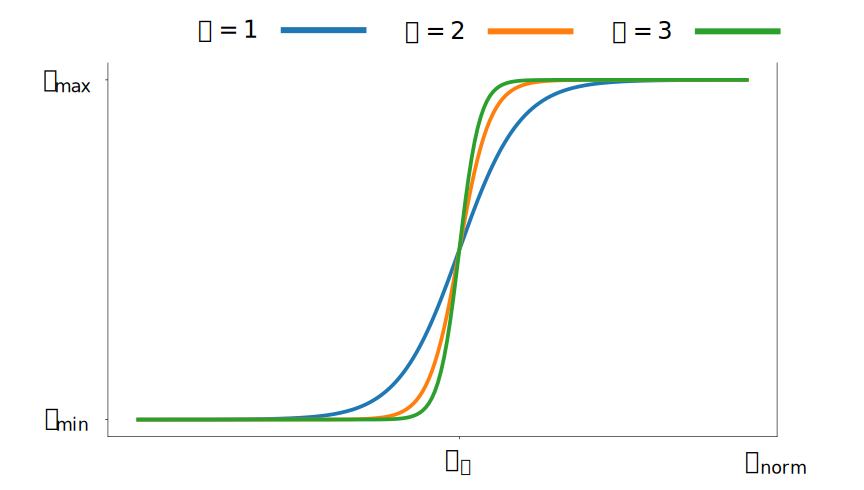
\includegraphics[width=\columnwidth]{figure/sigmoid_sensitivity.pdf}
    \caption{Sigmoid-based control function for loss shape parameter $\epsilon$}
    \label{sigmoid}
\end{figure}

\clearpage

\subsubsection{学習アルゴリズム}
アルゴリズム\ref{alg:proposed_method} に詳細なアルゴリズムを示す.
学習プロセスは難易度評価と損失パラメータ更新を行う適応的制御と,
実際にモデルパラメータを更新する学習段階の2つで構成される.

学習開始時,モデルパラメータ $\mathbf{W}$ を初期化し,全ての画像に対する損失形状パラメータ $\epsilon$ を $0$ に初期化する.
$E_0 > 0$の場合,エポック $1$ から $E_0 - 1$までの期間は初期学習期間とし,
$\epsilon=0$を固定して標準的なPolyDice-1 Lossで学習を行う.この期間により,モデルは不確実性推定に必要な基礎的な特徴表現を獲得する.
$E_0 = 0$の場合は,最初のエポックから適応的制御を開始する.

適応的学習期間($e \geq E_0$)では,$\tau$ エポックごとに適応的制御が実行される.
ここでは,3.2節で述べた手順に従い,MC Dropout推論による不確実性指標推定,画像単位への集約,正規化を経て,各画像の $\epsilon$ が更新される.
適応的制御の段階ではモデルパラメータ$\mathbf{W}$は固定されており,損失関数の形状パラメータ$\epsilon$の更新のみが行われることに注意されたい.

続く学習段階(Epoch $e$)では,更新された $\epsilon$ を用いてミニバッチ学習を行う.
具体的には,ランダムにサンプリングされたミニバッチを構成する画像のインデックス集合を $\mathcal{B} \subset \{1, \dots, N\}$ とする.
このとき,最適化の対象となる目的関数 $\mathcal{L}$ は,バッチ内の各画像 $n \in \mathcal{B}$ に個別に割り当てられた形状パラメータ $\epsilon_n$ を用いた PolyDice-1 Loss の平均として次式で定義される.

\begin{equation}
    \mathcal{L} = \frac{1}{|\mathcal{B}|} \sum_{n \in \mathcal{B}} \mathcal{L}_{\text{PolyDice-1}}(\hat{\mathbf{Y}}_n, \mathbf{Y}_n; \epsilon_n)
\end{equation}

ここで,$\mathcal{L}_{\text{PolyDice-1}}(\cdot; \epsilon_n)$ はパラメータ $\epsilon_n$ を適用した単一画像の損失関数を表す.
このように,バッチ内の各画像に対して異なる $\epsilon_n$ を適用することで,
難易度が高いと判定された画像には急峻な勾配を,低い画像には緩やかな勾配を同時に与えることが可能となる.
最終的に,この損失関数 $\mathcal{L}$ に基づく勾配降下法により,モデルパラメータ $\mathbf{W}$ が最適化される.
このサイクルを繰り返すことで,モデルの学習に応じて困難な画像の学習を重点的に行うことが可能となる.

\clearpage

\begin{algorithm}[t]
    \caption{Uncertainty-based Adaptive PolyDice-1 Loss Learning Algorithm}
    \label{alg:proposed_method}
    \begin{algorithmic}[1]
        \small
        \Require Training dataset $\mathcal{D} = \{(\mathbf{X}_n, \mathbf{Y}_n)\}_{n=1}^{N}$
        \Require Model $f_{\mathbf{W}}$, Max epochs $E$
        \Require \textbf{Hyperparameters:} Dropout probability $p$, Start epoch $E_0$, Interval $\tau$, MC iterations $T$, Normalization percentile $q$, Slope $k$, Range $[\epsilon_{\text{min}}, \epsilon_{\text{max}}]$
        
        \State Initialize model parameters $\mathbf{W}$
        \State Initialize loss parameters $\epsilon_n \leftarrow 0$ for all $n \in \{1, \dots, N\}$
        
        \For{$e = 1$ \textbf{to} $E$}
            \If{$e \geq E_0$ \textbf{and} $(e - E_0) \pmod \tau = 0$}
                \State Set model to evaluation mode (enable Dropout)
                
                \For{$n = 1$ \textbf{to} $N$}
                    \For{$t = 1$ \textbf{to} $T$}
                        \State $\hat{\mathbf{Y}}^{(t)} = f_{\mathbf{W}}(\mathbf{X}_n; \mathbf{z}^{(t)}), \quad \mathbf{z}^{(t)} \sim \text{Bernoulli}(1-p)$
                    \EndFor
                    
                    \State Calculate pixel-wise Mutual Information (Eq. 9):
                    \State $I_{n, i,j} = H\left( \frac{1}{T} \sum_{t=1}^{T} \hat{y}_{n, i,j}^{(t)} \right) - \frac{1}{T} \sum_{t=1}^{T} H\left( \hat{y}_{n, i,j}^{(t)} \right)$
                    
                    \If{positive region $\mathcal{P}_n \neq \emptyset$}
                        \State Compute $\mu_{\mathcal{P}_n}, \sigma_{\mathcal{P}_n}$ from $\{I_{n,i,j} \mid (i,j) \in \mathcal{P}_n\}$
                        \State Identify valid pixels: $\mathcal{P}_n' = \{(i,j) \in \mathcal{P}_n \mid |I_{n,i,j} - \mu_{\mathcal{P}_n}| \leq 2\sigma_{\mathcal{P}_n} \}$
                        \State $D_n = \frac{1}{|\mathcal{P}_n'|} \sum_{(i,j) \in \mathcal{P}_n'} I_{n, i,j}$
                    \Else
                        \State $D_n \leftarrow 0$ \Comment{Handle negative samples}
                    \EndIf
                \EndFor

                \State \textbf{Step 2: Normalization \& $\epsilon$ Update}
                \State Compute $q$-percentile $D_q$ and std $\sigma_D$ from $\{D_n\}_{n=1}^N$
                \For{$n = 1$ \textbf{to} $N$}
                    \State Normalize score (Eq. 13): $D_{n, \text{norm}} = \frac{D_n - D_{q}}{\sigma_D + \delta}$
                    \State Update $\epsilon_n$ (Eq. 14): $\epsilon_n \leftarrow \epsilon_{\text{min}} + (\epsilon_{\text{max}} - \epsilon_{\text{min}}) \sigma(k \cdot D_{n, \text{norm}})$
                \EndFor
            \Else
                \State \Comment{Keep current $\epsilon_n$ (Note: $\epsilon_n=0$ if $e < E_0$)}
            \EndIf

            \State
            \State Set model to training mode (disable MC Dropout)
            \For{each minibatch $\mathcal{B} \subset \{1, \dots, N\}$}
                \State Compute batch loss with sample-specific $\epsilon_n$ (Eq. 15):
                \State \quad $\mathcal{L} = \frac{1}{|\mathcal{B}|} \sum_{n \in \mathcal{B}} \mathcal{L}_{\text{PolyDice-1}}(\hat{\mathbf{Y}}_n, \mathbf{Y}_n; \epsilon_n)$
                \State Update parameters: $\mathbf{W} \leftarrow \mathbf{W} - \eta \nabla_{\mathbf{W}} \mathcal{L}$
            \EndFor
        \EndFor
        \State \Return Trained parameters $\mathbf{W}$
    \end{algorithmic}
\end{algorithm}

\clearpage